\documentclass[article,type=msc,colorback,12pt,accentcolor=tud7b]{tudthesis}
\usepackage{ngerman}
\usepackage[english]{babel}
\usepackage{cite}
\graphicspath{ {images/} }


\newcommand{\getmydate}{%
  \ifcase\month%
    \or Januar\or Februar\or M\"arz%
    \or April\or Mai\or Juni\or Juli%
    \or August\or September\or Oktober%
    \or November\or Dezember%
  \fi\ \number\year%
}

\begin{document}
  \thesistitle{Feedback Driven Development of Cloud Applications} 
  %\linebreak[1]Corporate-Design f"ur {\LaTeX}!}%
    {Feedback Driven Development of Cloud Applications}
  \author{Harini Gunabalan}
  \birthplace{}
  \referee{Prof. Dr.-Ing. Mira Mezini}{Dr. Guido Salvaneschi}
  \department{Department of Computer Science}
  \group{Software Technology Group}
  \dateofexam{31 May 2015}{31 May 2015}
  \tuprints{12345}{1234}
  \makethesistitle
  \affidavit{Harini Gunabalan}


\begin{abstract}
\begin{large} 
	
\par Over the last few years, the Cloud Computing Paradigm has gained a lot of importance in both the Academia and the Industry. The cloud has not only changed the IT Landscape from the user's perspective but has also changed how the Developers develop applications on the cloud. The increasing adoption of the DevOps approach has led to the removal of the boundaries between the development and the operations. 



\par Among the the three levels of the Cloud Computing: Infrastructure-as-a-Service (IaaS), Platform-as-a-Service(PaaS) and Software-as-a-Service(SaaS), Software Developers are mainly concerned with the PaaS which allows them to focus on the Application Development. Leveraging the fact that the Application is hosted on the cloud, there are additional metrics regarding the application available to Developers in different Log formats. There are also Cloud Monitoring Tools which consolidates these logs with a huge volume of data representing the run-time metrics etc. of the cloud applications. Though monitoring of the cloud applications has been done by many tools, most of the developers do not go through the cumbersome error/warning log data.These log data are not visually made available to the developers in their Development Environment. By providing this information, developers can have an overview of the Application Performance at real time, and can capture issues that occur at scale which normally could not be captured by Profilers. This could also help us to reduce the developer-operator gap providing an improved DevOps experience. 

\par This Thesis work aims in addressing this issue. The focus is mainly to map the run-time metrics to the source code artifacts, thereby helping the developers link the Run time metrics to the source code. Mapping will involve log data aggregation, code analysis techniques etc.

	
\end{large}
\end{abstract}  

\clearpage

%=====INDEX================================================================================
\setlength{ \parskip }{1em}
\index{key}
\tableofcontents 
\cleardoublepage 

\listoffigures
\clearpage
\appendix
\cleardoublepage 

% abstract, acknowledgements, contents
 \section{Introduction}
	
	Cloud Computing is one of the fields in Computer Science that has gained rapid growth and importance in the recent years. The fact that the servers are remote hosted rather than local servers has led to innumerable small scale businesses. Start-ups no longer require high infrastructure, instead they just need to pay for the amount of resources that they actually use (pay-per-use). This also significantly reduces the initial monetary setup costs for such start-ups. There has been extensive research in Cloud Computing areas such as auto-scaling of resources at the infrastructure level, monitoring of metrics at both the application and infrastructure level. However, there is not much research done in how these monitored metrics are utilized by the Cloud Application Developers. Making the run-time metrics visibly effective for the developers in their Development Environment is the issue this thesis is aiming to solve.
	\par This chapter is structured into four sections. The first section provides the motivation of this thesis work. The second section gives an insight into the problem statement which this Thesis work aims to solve. The third section details the contribution of the work and the fourth section provides how the following chapters of the Thesis are structured.
	
	\subsection{Motivation}
	
	Software Engineering Practice in the industry has faced a phenomenal change since the advent of Cloud Computing. This is mainly due to the flexibility and the dynamic scaling up and scaling down of the infrastructure as required by the current workload. This proves not only to be elastic but cost-effective as well. It is quite obvious that this elasticity is achieved by the continuous monitoring of several metrics that indicate the demand at the moment, and provisioning the necessary resources to meet the monitored demand. Distributed, scalable enterprise-wide applications also mandate the monitoring of metrics for reasoning the effectiveness of the applications by engineers and business analysts \cite{leitner2012application}.
	
	\par The metrics that are being monitored vary widely. For instance, the metrics such as memory consumption, CPU utilization, Network bandwidth utilization could be considered to be at the Infrastructure level, whereas some other metrics such as Response times of methods/procedures, the number of users accessing the application, maximum number of users who can use the application simultaneously, etc. could be considered to be at the application level. Sometimes, the application level metrics could depend on the primitive metrics at the infrastructure level and vice-versa.
	
	\par As Cloud Application Development has becoming more common, the run time monitoring metrics of these applications are available through several Application Performance Monitoring (APM) tools such as Amazon Cloudwatch, New Relic, etc. But, they do not provide any valuable and visible feedback to the developers, and hence most of the cloud developers do not use it. However, this run-time monitoring data could be used to provide useful analytic information such as performance hotspots that is taking a lot of execution time, and predictive information such as methods or loops that may become critical, even before the deployment. This type of analytic and predictive feedback should be provided to the developers in their IDEs which otherwise may not be explored by the developers. This technique of utilizing the monitoring data is known Feedback driven development. Feedback Driven Development that provides visual tools to the cloud developers is the focus of this thesis research.	
	
	\subsection{Problem Statement}	
	
The Cloud computing paradigms are classified into three service models which forms a stack as shown in Figure A.1 

\begin{center}
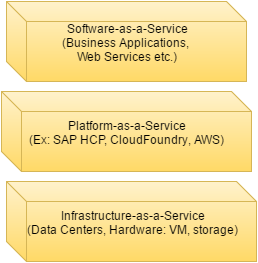
\includegraphics[scale=0.7]{A1}
\end{center}

%\begin{itemize}
%	
%	\item Infrastructure-as-a-Service
%	
%	\item Platform-as-a-Service
%	
%	\item Software-as-a-Service  
%% add the stack image 	
%\end{itemize}
	
\cite{bruneo2015framework} defines a framework that collects data as defined by a 3-D cloud monitoring model. From the software engineering perspective, it is important to note how Cloud Computing impacts the development practices. Based on the research conducted, there are two important research issues \cite{cito2014making}. 

\begin{itemize}

	
	\item Impact of DevOps on Cloud Application Developers:	
	The Cloud Developers are forced to look into the huge log data of the cloud applications. Development and Operations are brought much closer than the traditional software methods. Sometimes the same person acts as both the developer and the operator. 
	
	\item Data and Tools utilized by Cloud Developers:
	The data produced by the logs include Business Metrics, System-level Data etc. Sometimes the implementation changes may even have monetary consequences in the cloud, nevertheless most of the developers do not pay attention to this aspect. Hence it can be argued that once these operational metrics are brought closer to the Cloud Developers Environment, they would be able to pay closer attention to this information thereby achieving cost-effective applications.
	
\end{itemize}

Considering these issues, it is certainly important how we are going to leverage these Cloud monitoring Logs to make a useful impact for the Cloud Developers. 
 
 	\subsubsection{Continuous Delivery in Cloud Development}
 	As we compare the software development on-premise with that of the Cloud, there has been a huge change in every software release. Deployment cycles has been reduced from months to days and sometimes even within a few hours the next version is released. This process is often referred to Continuous Delivery(CD) in the Cloud Computing terms. Most companies make use of this Continous Delivery to rollout new features and evaluate their new ideas in a controlled manner \cite{kohavi2007practical}. CD has become a huge success and companies such as Google,Facebook etc. adopt CD of varying degrees for some of their services. When a feature is delayed for the current roll-out, it gets delayed by months when the traditional software development life-cycle is used. The feature needs to be delayed until the next release. Whereas in this CD approach the next release could be in the same day or in the same week, leading to small changes of production code. This also leads to a state called "perpetual development" where the code is always under continuous development and there is no stable release version for a particular product.  	\par Owing to this new release paradigm, there are a lot of extra information generated. The live performance of the application, click-streams from the User Interface of application, error and warning logs, infrastructure related data etc. are produced. There are a lot of existing APM Tools that collect this data and generate information out of it, however, how this information could be made effective to the software developers in their daily routine is a topic that is not discussed very often. 
 	
 	\subsubsection{Monitoring Metrics: Scalability and Availability of the Application}
 	
	Some of the monitoring metrics collected include the CPU usage, response time of the request, number of instances the application is hosted on, no. of requests each instance serves during a particular time period, error logs of the request etc. While these metrics focus mainly at the Infrastructure level, the logs instrumented into the application are also collected. We use these metrics to focus on two main challenges of cloud computing: Scalability and Availability of the Cloud applications.
	
	\par Scalability is the ability to increase or decrease the resources of an instance or the number of instances so that the changing demand of the incoming requests can be met. The platform related log data are collected for both Horizontal scaling (increasing the number of instances) and Vertical scaling(increasing the resources of each instance).
	
	\par Availability is one of the major goals of Cloud Computing. It means that the Cloud Services need to be available and accessible at anytime from anywhere. For business to happen continuously, it is necessary for the services to be highly available. The definition of availability is specified by the different Cloud vendors in their SLAs. For example, Google Search is known for its high availability.	
	
	\subsubsection{Incorporating the collected Feedback in the Development Environment}	
	
	Using the collected metrics, in this thesis, we aim to provide an efficient feedback to the Cloud Developers. The collected feedback is integrated into the Development Environment (IDEs) so that developers are able to utilize the feedback to make their applications better scalable and highly available.	
	
	
	\subsection{Contribution}
	
	\subsection{Structure of the Thesis}

	\par This thesis is structured in six chapters. Chapter 1 provides a short introduction into the topic and describes the goals of the thesis. Chapter 2 includes more background information and presents the state of the art of the important topics of this thesis: Cloud Application Performance Monitoring(AMP) tools, Feedback Driven Development(FDD) in general, and how FDD could be useful for Cloud Application Developers. The third Chapter describes an overview of the high-level System Design and the design decisions made in this research work. The fourth chapter explains the system on a lower fine-grained level. Interesting Implementation details are also provided here. Chapter 5 shows the various case studies, evaluates the developed system and illustrates its usage as well as possible applications. Finally, Chapter six provides the conclusion of the thesis and outlines the future work ideas.

% Example of Footnote    
%     \textbf{Alle Vordefinierten Texte sind, wie verbindlich vorgeschrieben, in der hessischen Amtssprache
%    gehalten\footnote{Deutschland hat (noch) keine Amtssprache.}.}

	\cleardoublepage

 \section{State of the Art}
 	
	This chapter presents the state of art of the topics relevant for this thesis. In the first section, we introduce Feedback Driven Development(FDD) and the types of FDD. The second section focuses on the Log Structure, Metrics and the libraries that are consolidated to provide the feedback.  
 	
	\subsection{Feedback Driven Development } 		
	
	When an application is deployed in the Cloud, normally a lot of monitoring data is collected. This can be broadly classified into: Application Level Logs and Infrastructure Level Logs. This data could be made useful to both the Developers and Operators. Infrastructure Logs provides details such as number of instances, the memory, CPU, Disk utilization of each instance, which instance serves a particular request etc. By making this kind of data visible to the developers, they can tweak the application development process, as they have access to the cloud internal systems. At the same time, the Cloud operators also benefit with the relevant business metrics to manage the instances more efficiently. 
	
	\par Collecting these run-time data, aggregating them into useful feedback, and feeding them back into the Development process of an application could create a useful impact in the future deployment of the application. This process is known as Feedback Driven Development(FDD). FDD can be classified into 2 types: Analytic FDD and Predictive FDD \cite{cito2015runtime}.
	
	\subsubsection{Analytic FDD}
		
	Analytic FDD is that data which is brought directly into the developer environment. It provides a mapping between the log data collected and the source code artifacts. This helps the developers to understand how the run-time metrics directly impact the source code. Based on this developers can alter and optimize the code based on the real time user behavior. In practice, Analytic FDD deals with visualizing the run time operations data and how it is being mapped to the code artifacts. 
		
	\subsubsection{Predictive FDD}
Predictive FDD is one step ahead compared to the Analytic FDD. It utilizes the run-time feedback to warn the developers about the current code changes even before the updated source code is deployed. Predictive FDD is combined with static code analysis to give better predictions regarding a code change. 


 		
	\subsection{Logging}
		
		As depicted in \cite{jiang2009understanding} , it is clear that Auto Generated issues are resolved much faster than human generated issues. Auto generated issues are those that have attached symptoms and system logs as event messages, whereas Human generated issues are those reported by the users usually through email tickets/phone calls. This further justifies the use and necessity of logging. \cite{jiang2009understanding} also lists down the challenges of using the logging information.
		
		The Log Data collected to generate the feedback is discussed here. Among the two types of data: Monitoring Data and Production data as detailed in \cite{cito2015runtime} we focus on the Monitoring data. This category of data is further classified as Load Data (incoming requests, server utilization, number of instances), Performance data (Response times, hotspots), cost data and User Behavior Data (Click Streams). This data is mostly collected by existing APM Tools.
		
		\cite{yuan2012conservative} answers the question of where to add logs proactively that could help minimize the effort of failure diagnosis. ERRLOG, a tool that identifies in which location log needs to be added is developed. Errlog makes use of code analysis techniques to achieve this. iTrack, a framework for monitoring user activities and correlating them with system data is done to detect service outages as in \cite{mann2011correlating}. 
			
	\subsubsection{Logging Tools and Metrics}	

		\subsubsection{Log Structure}	
		
		\subsubsection{Performance related Logging}
		\cite{nagaraj2012structured} explains a tool known as DISTALYZER that analyses the system logs to identify the performance issues. This tool analyses logs from large scale distributed systems and compares a set of baseline logs with an acceptable performance with another set of logs with unacceptable performance. DISTALYZER uses machine learning techniques which first creates a set of features(event/state variables) for the logs. Further Predictive and Descriptive Modeling are performed on these variables to provide the developers the root cause of the issue.
		
		
		
		\subsubsection{Click Stream Logging}
	
	
	
 \cleardoublepage
 \section{System Design}	
 \subsection{System Design}

 \cleardoublepage
 \section{System Implementation}
 \subsection{System Implementation}

 \cleardoublepage	  
 \section{Evaluation and Results}	  
 \subsection{Evaluation}
 
 \cleardoublepage
 \section{Conclusion and Future Work}	  
 \subsection{Conclusion and Future Work}

\clearpage
	  
%=====BIBLIOGRAPHY================================================================================
\bibliographystyle{plain}
\bibliography{LatexRefThesis}	  

\end{document}
